\documentclass[10pt]{article}

\usepackage[T1]{fontenc}
\usepackage[utf8]{inputenc}
\usepackage{newtxtext,newtxmath}
\usepackage[letterpaper,margin=0.85in]{geometry}
\usepackage{microtype}
\usepackage{graphicx}
\usepackage{booktabs,array,tabularx}
\usepackage{ragged2e}
\usepackage{xcolor}
\usepackage{hyperref}
\usepackage{caption}
\usepackage{enumitem}
\usepackage{amsmath}
\usepackage{titlesec}
\usepackage{abstract}
\usepackage{placeins}
\usepackage{rotating}

\definecolor{LinkBlue}{HTML}{1A5599}
\definecolor{NoteGray}{HTML}{6B6B6B}
\definecolor{WarnRed}{HTML}{8B1A1A}
\hypersetup{colorlinks=true,linkcolor=LinkBlue,citecolor=LinkBlue,urlcolor=LinkBlue,
  pdftitle={Phase-resolved spatial attention in a noisy-memory Luo-Maunsell change-detection agent},
  pdfauthor={Jonathan Morgan}}
\graphicspath{{../figures/}}

\captionsetup{font=small,labelfont=bf,justification=justified,singlelinecheck=false,skip=4pt}
\setlist{nosep,leftmargin=1.2em}
\setlength{\parindent}{1em}
\raggedbottom
\emergencystretch=2em

\titleformat{\section}{\normalfont\large\bfseries}{\thesection}{0.7em}{}
\titleformat{\subsection}{\normalfont\bfseries}{\thesubsection}{0.7em}{}
\titlespacing*{\section}{0pt}{1.1em}{0.5em}
\titlespacing*{\subsection}{0pt}{0.9em}{0.4em}

\renewcommand{\abstractnamefont}{\normalfont\bfseries\large}
\renewcommand{\abstracttextfont}{\normalfont\small}

\newcommand{\env}[1]{\texttt{#1}}
\newcommand{\note}[1]{\textcolor{NoteGray}{\textit{#1}}}
\newcolumntype{Y}{>{\RaggedRight\arraybackslash}X}

\begin{document}

{\centering
{\LARGE\bfseries Where does attention go, and when?\par}
\vspace{4pt}
{\large\bfseries Phase-resolved spatial routing in a noisy-memory\\[2pt]
Luo--Maunsell change-detection agent\par}
\vspace{10pt}
{\large Jonathan Morgan\par}
\vspace{2pt}
{\small RViT$+$ attention evidence program \quad$\cdot$\quad 4 August 2026\par}
\vspace{12pt}
}

\begin{abstract}
\noindent
A recurrent vision transformer with a noisy spatial recurrent memory (mnemonic noise
SD $0.64$) was trained by reinforcement learning on a seven-frame analogue of the
Luo and Maunsell (2015) two-location orientation change-detection task, which contains no
spatial cue. We re-express the frozen checkpoint's cross-attention weights in the
common-quadrant convention used throughout our value-directed-attention (VDA) series and
resolve them jointly by \emph{frame} and by \emph{environment condition}
(changed vs.\ unchanged first test $\times$ tested location L0 vs.\ L3), holding the latent
trial fixed and averaging only over $64$ repetitions of sensory and mnemonic noise. Three
results follow. (i) The two key sources dissociate completely: the visual-key map is
\emph{identical in all four conditions at every frame} and is governed only by which
patches contain a Gabor, which it consistently \emph{avoids}
($0.215$ vs.\ $0.285$ conditional quadrant mass during the samples; $0.201$ vs.\ $0.267$ at
the tests). (ii) All time-varying, condition-contingent selectivity lives in the
recurrent-memory keys, which follow a four-stage encode $\rightarrow$ maintain $\rightarrow$
reset $\rightarrow$ select sequence: uniform at $t_0$, split across both sample quadrants at
$t_1$--$t_2$, returned to near-uniform at first-test onset $t_3$, and concentrated on the
tested location at $t_4$ ($0.49$--$0.57$ vs.\ $0.14$--$0.17$) and through the gap $t_5$
($0.84$--$0.91$). (iii) That selection is not location-general: at the guaranteed second
test $t_6$ memory routing collapses onto a \emph{fixed} quadrant (L0, $0.70$ in both
conditions), so the tested-minus-other contrast reverses sign between the two tested
locations ($+0.194$ vs.\ $-0.188$). Memory keys carry only $1$--$14\%$ of the joint softmax,
and that share tracks the number of visible Gabors ($0.010$ blank, $0.075$ one, $0.140$ two)
rather than the task phase. A companion suppression experiment drove sample-phase mass at
the future-tested quadrant from $0.234$ to $0.001$ with zero discordant trials in $704$
matched pairs, so none of this routing is shown to be response-causal.
\textcolor{WarnRed}{\textbf{Validity:} the checkpoint predates a corrected orientation-sampling
contract and is retained for forensic provenance only (Section~\ref{sec:validity}). This is
a measurement and display report, not an admissible behavioural or biological claim.}
\end{abstract}

\vspace{6pt}

\section{Introduction}

Luo and Maunsell (2015) dissociated attention-driven changes in \emph{sensitivity} from
changes in \emph{criterion} by counterphasing the reward schedule across two stimulus
locations in an orientation change-detection task that contains no visual cue. The task is
attractive as a model system precisely because selection must be endogenous: both sample
Gabors are simultaneously task-relevant, and nothing in the display tells the observer which
location will be tested.

Our VDA series has so far studied \emph{cued} change detection, where a spatial cue supplies
a named location to which routing weights can be aligned. This report asks the
complementary question in the uncued Luo task: in a trained agent, where does attention go
at each frame, and does that allocation differ across the environment conditions the agent
actually experiences? We measure the same quantities and use the same display convention as
the VDA figures --- a common physical $2\times2$ partition of the native key grid, key
sources split before any query reduction, and uniform-normalized quadrant scores --- so that
the uncued and cued results are directly comparable.

The contribution is a measurement, not a mechanism. We show that in this checkpoint the
visual and recurrent-memory key blocks play completely different roles, that the memory
block alone carries the phase-resolved spatial signal, and that its apparent
``return to the tested site'' fails a location-generality control. We also report the
negative causal result that accompanies it.

\section{Methods}

\subsection{Task}

The environment (\env{luo2015\_criterion}) is a scaled seven-frame analogue of the published
protocol. Two Gabors occupy diametrically opposed locations of a logical $2\times2$ grid,
top-left (L0) and bottom-right (L3). Frames $t_0$--$t_1$ present both samples; $t_2$ is a
blank delay; $t_3$--$t_4$ are the first-test response window at one randomly chosen location;
$t_5$ is an inter-test gap; and $t_6$ is a guaranteed changed second test, presented only on
trials whose first test was unchanged (Figure~\ref{fig:task}). Declaring during $t_3$--$t_4$
scores a hit or a false alarm; withholding is verified by requiring a declaration to the
second test. There is no cue at any point. Sensory orientation noise is
$5.0^\circ$ per drawn Gabor.

\subsection{Model and checkpoint}

The agent is a recurrent vision transformer with a convolutional front end, a $20\times20$
patch grid over a $50\times50$ scene, an xLSTM spatial recurrent memory of width
$d_\mathrm{mem}=32$ with decay $1.0$ and additive mnemonic noise of SD $0.64$, and an
actor--critic head with two actions (wait, declare). Routing is \env{crossattn1}: current
visual tokens supply the queries while visual tokens and recurrent-memory tokens jointly
supply keys and values in a single softmax, so the key axis has $2\times400=800$ entries
split into a $400$-token visual block and a $400$-token memory block. All results come from
one frozen mid-training checkpoint (iteration $12{,}899$, SHA-256 \texttt{2c4a6d2d\dots}),
copied and hashed before analysis. Nothing was retrained or re-run for this report; the
figures re-express arrays cached by the 2026-08-03 scientific assay.

\subsection{Attention measurement and display convention}

Let $A$ be one trial's $400\times800$ attention matrix at a named frame. Following the
source-separated convention already used for VDA4, VDA16 and the spatial-scaling battery, we
split the visual and memory key blocks \emph{before} averaging over queries and before any
spatial reduction. Averaging over queries gives per-source incoming token mass; summing that
over each of the four quadrants of the $20\times20$ grid gives a source share $w_s$
(the fraction of the joint softmax landing on source $s$, with $w_V+w_M=1$) and, dividing by
$w_s$, a \emph{source-conditional quadrant total} that sums to one within each source. The
uniform baseline for that score is therefore $0.25$ per quadrant regardless of source, which
is what makes the panels in Figures~\ref{fig:visual}--\ref{fig:memory} comparable across
frames, conditions and sources. We separately report query-resolved routing: the mass sent
from the tested-location query quadrant to the same versus the other sample quadrant, within
each source.

\subsection{Conditions and trial construction}

The design crosses first-test change status (changed, unchanged) with tested location
(L0, L3), giving four environment conditions. Within each condition the latent trial is held
fixed --- same sample orientations, same tested location, same $+18^\circ$ signed
change --- and the only variation across the $64$ trials per cell is the sensory and
mnemonic noise. Policy actions are sampled, not argmaxed. Changed trials terminate inside the
first-test window (declaration, or a miss at the end of $t_4$), so frames $t_5$--$t_6$ are
never experienced on those trials and are shown greyed out rather than averaged in. This is
the survivor control that a naive frame-averaged map silently violates.

\begin{figure}[t]
\centering
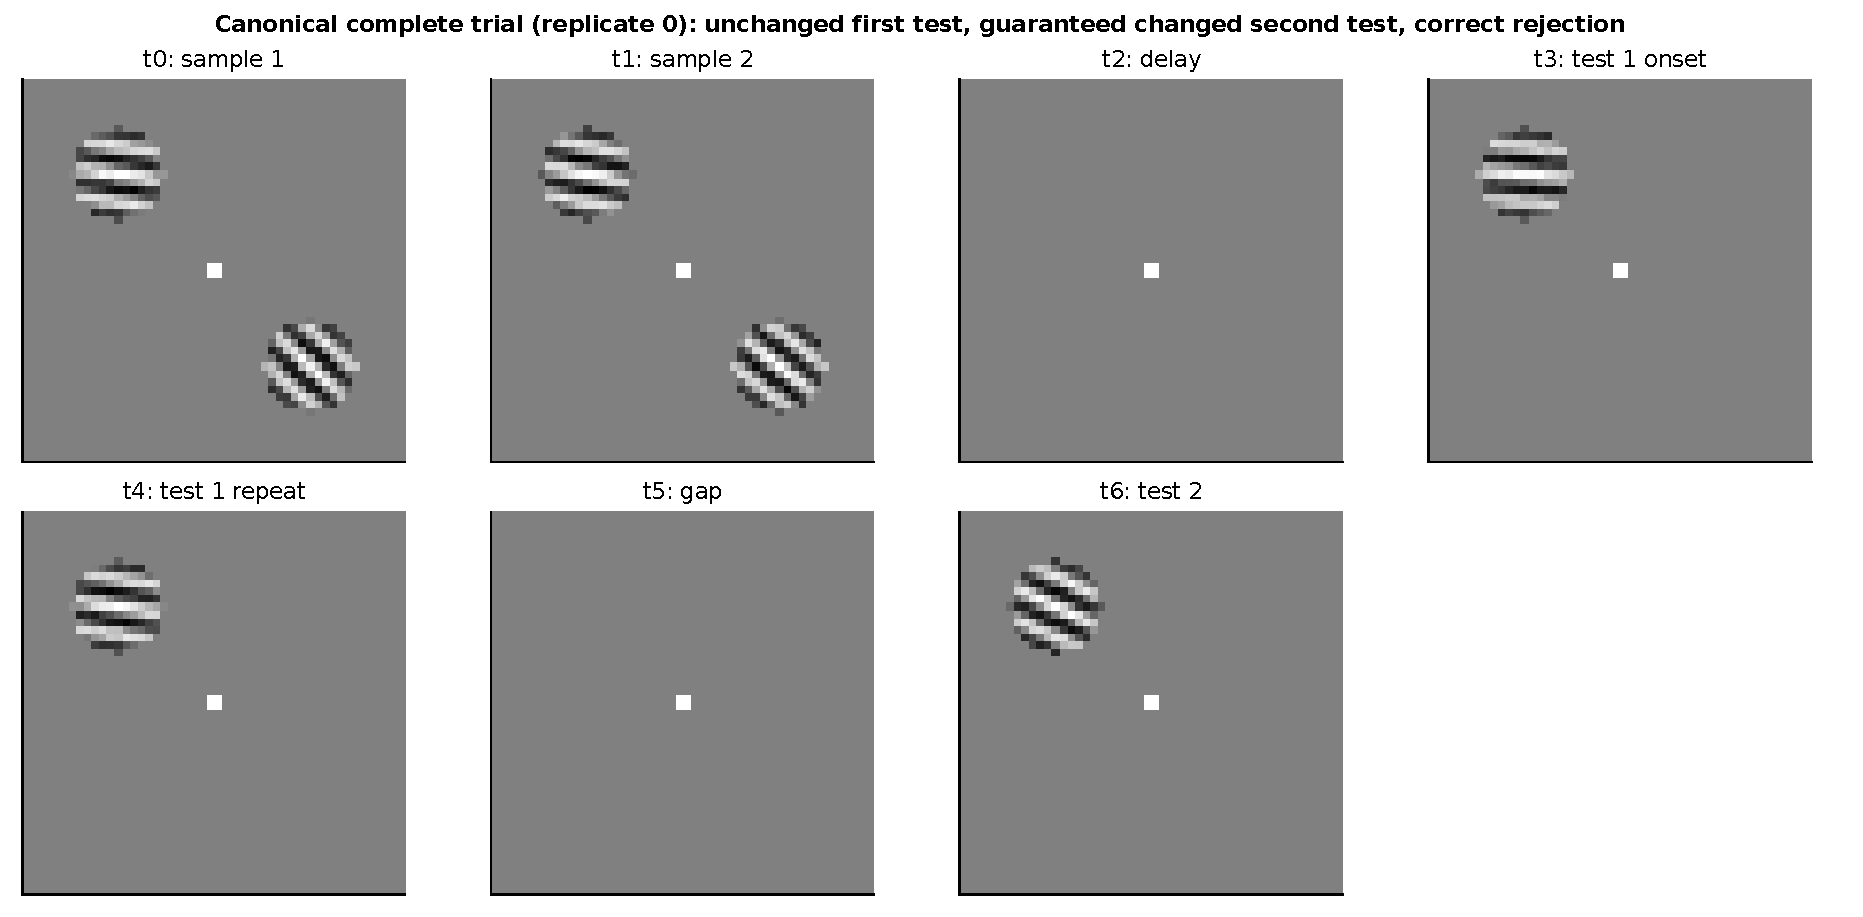
\includegraphics[width=\textwidth]{task_trial_montage.pdf}
\caption{\textbf{The seven-frame uncued task.} A complete unchanged-first-test trial ending
in a correct rejection at the guaranteed changed second test. Both samples appear at
$t_0$--$t_1$; the delay $t_2$ and gap $t_5$ are blank; one location is tested at $t_3$--$t_4$
and again at $t_6$. No cue appears at any frame.}
\label{fig:task}
\end{figure}

\section{Results}

\subsection{Behaviour of the frozen checkpoint}

On the fixed $+18^\circ$ probe used for all attention figures the checkpoint is
near ceiling: $63/64$ and $64/64$ hits at L0 and L3, and $60/64$ and $59/64$ correct
rejections, i.e.\ $246/256$ ($0.961$) correct. Across the full controlled magnitude ladder
natural accuracy is $476/704$ ($0.676$). The psychometric function is non-monotonic
(Figure~\ref{fig:behaviour}): hit rate and $d'$ peak at $18^\circ$
($0.984$, $d'=3.44$) and fall to $0.547$ and $d'=1.57$ at $35^\circ$, while the
criterion $c$ falls to $-0.30$ at $18^\circ$ and rises again to $+0.66$ at
$35^\circ$. Because sensitivity and criterion move together at the large-change end,
the decline is not attributable to sensitivity alone, and we do not offer a mechanism for it
here. \note{These are controlled fixed-magnitude slices within the training support, not the
training distribution; each point is $64$ changed trials against $128$ shared no-change
trials from one checkpoint.}

\begin{figure}[t]
\centering
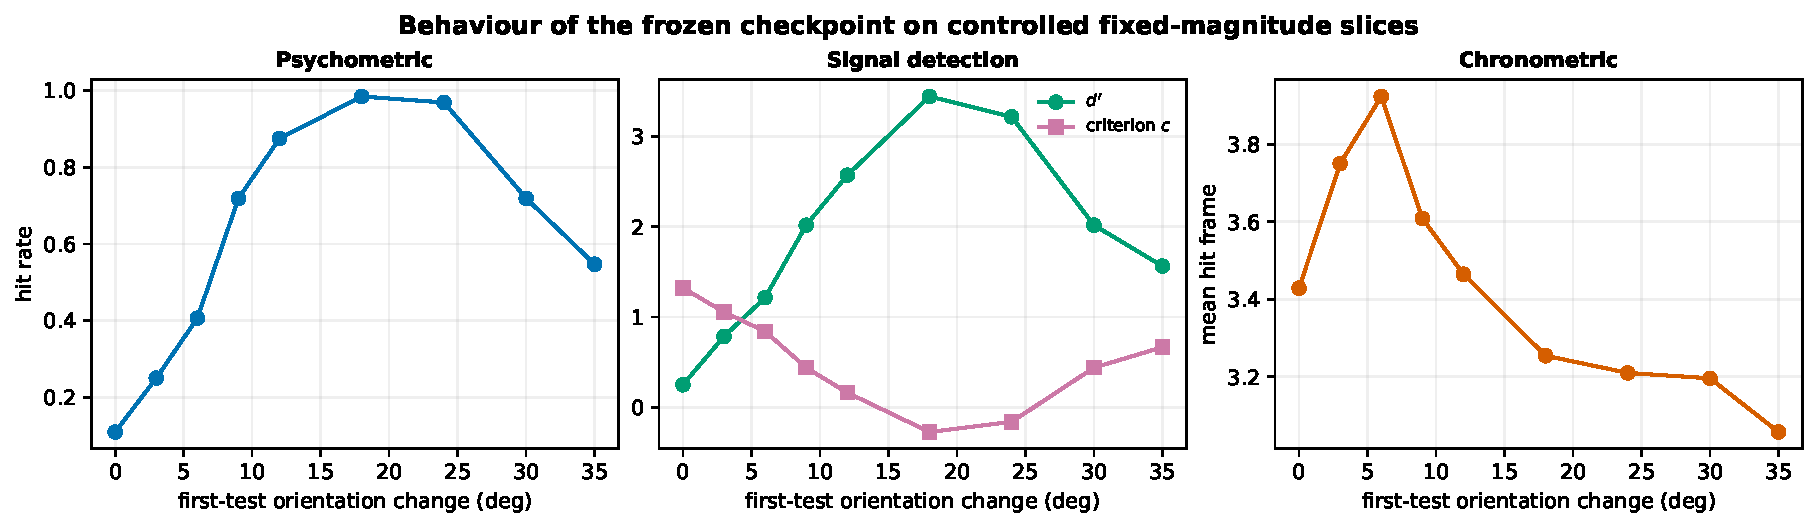
\includegraphics[width=\textwidth]{behaviour_curves.pdf}
\caption{\textbf{Behaviour on controlled fixed-magnitude slices.} Hit rate, signal-detection
decomposition, and mean hit frame as a function of first-test orientation change. Sensitivity
peaks at $18^\circ$ --- the probe used for every attention figure --- and both $d'$
and $c$ degrade at the largest changes.}
\label{fig:behaviour}
\end{figure}

\subsection{Key-source share tracks visible stimuli, not task phase}

Memory keys receive a small and highly structured minority of the joint softmax. Their share
$w_M$ is $0.140$ at $t_0$--$t_1$, $0.010$ at $t_2$ and $t_5$, and $0.075$ at $t_3$, $t_4$
and $t_6$ (middle row of Figure~\ref{fig:timecourse}). These three values correspond exactly
to two visible Gabors, none, and one. The share is identical in all four conditions to three
decimals. \textbf{The visual/memory balance is therefore a function of how much stimulus
energy is on the screen, not of what stage of the trial the agent is in} --- the delay and
the gap are indistinguishable to it, as are the first and second tests. Any statement about
memory-key selectivity below is conditional on a source that never exceeds $14\%$ of the
total mass.

\subsection{Visual keys: one fixed map that avoids the stimuli}

The source-conditional visual map (Figure~\ref{fig:visual}) is remarkable for what it does
\emph{not} do. Its four quadrant values are the same in all four conditions at every frame,
to two decimals, and they depend only on which patches currently contain a Gabor:

\begin{itemize}
\item Both samples present ($t_0$, $t_1$): stimulus quadrants $0.215$, blank quadrants
$0.280$ and $0.290$.
\item Blank frames ($t_2$, $t_5$): $0.250$ everywhere, i.e.\ exactly uniform.
\item One Gabor present ($t_3$, $t_4$, $t_6$): tested quadrant $0.201$, the other three
$0.267$.
\end{itemize}

\vspace{6pt}
\noindent The sign is consistent and against the naive expectation: incoming visual-key attention is
\emph{lower} at occupied locations than at empty ones, by $0.065$--$0.066$ of conditional
quadrant mass. The query-resolved version is equally rigid --- the tested-location query
sends $0.048$ \emph{less} visual mass to its own quadrant than to the other one, at every
test frame in every condition (bottom row of Figure~\ref{fig:timecourse}). This reproduces,
in the common-quadrant display, the negative sample-stimulus-minus-blank
($-0.031$) and first-test target-minus-other ($-0.048$) contrasts previously reported for
this checkpoint. A visual routing block that is invariant to change status, invariant to
tested location, and inversely related to stimulus presence is better described as a fixed
contrast-dependent normalization than as spatial selection.

\begin{sidewaysfigure}
\centering
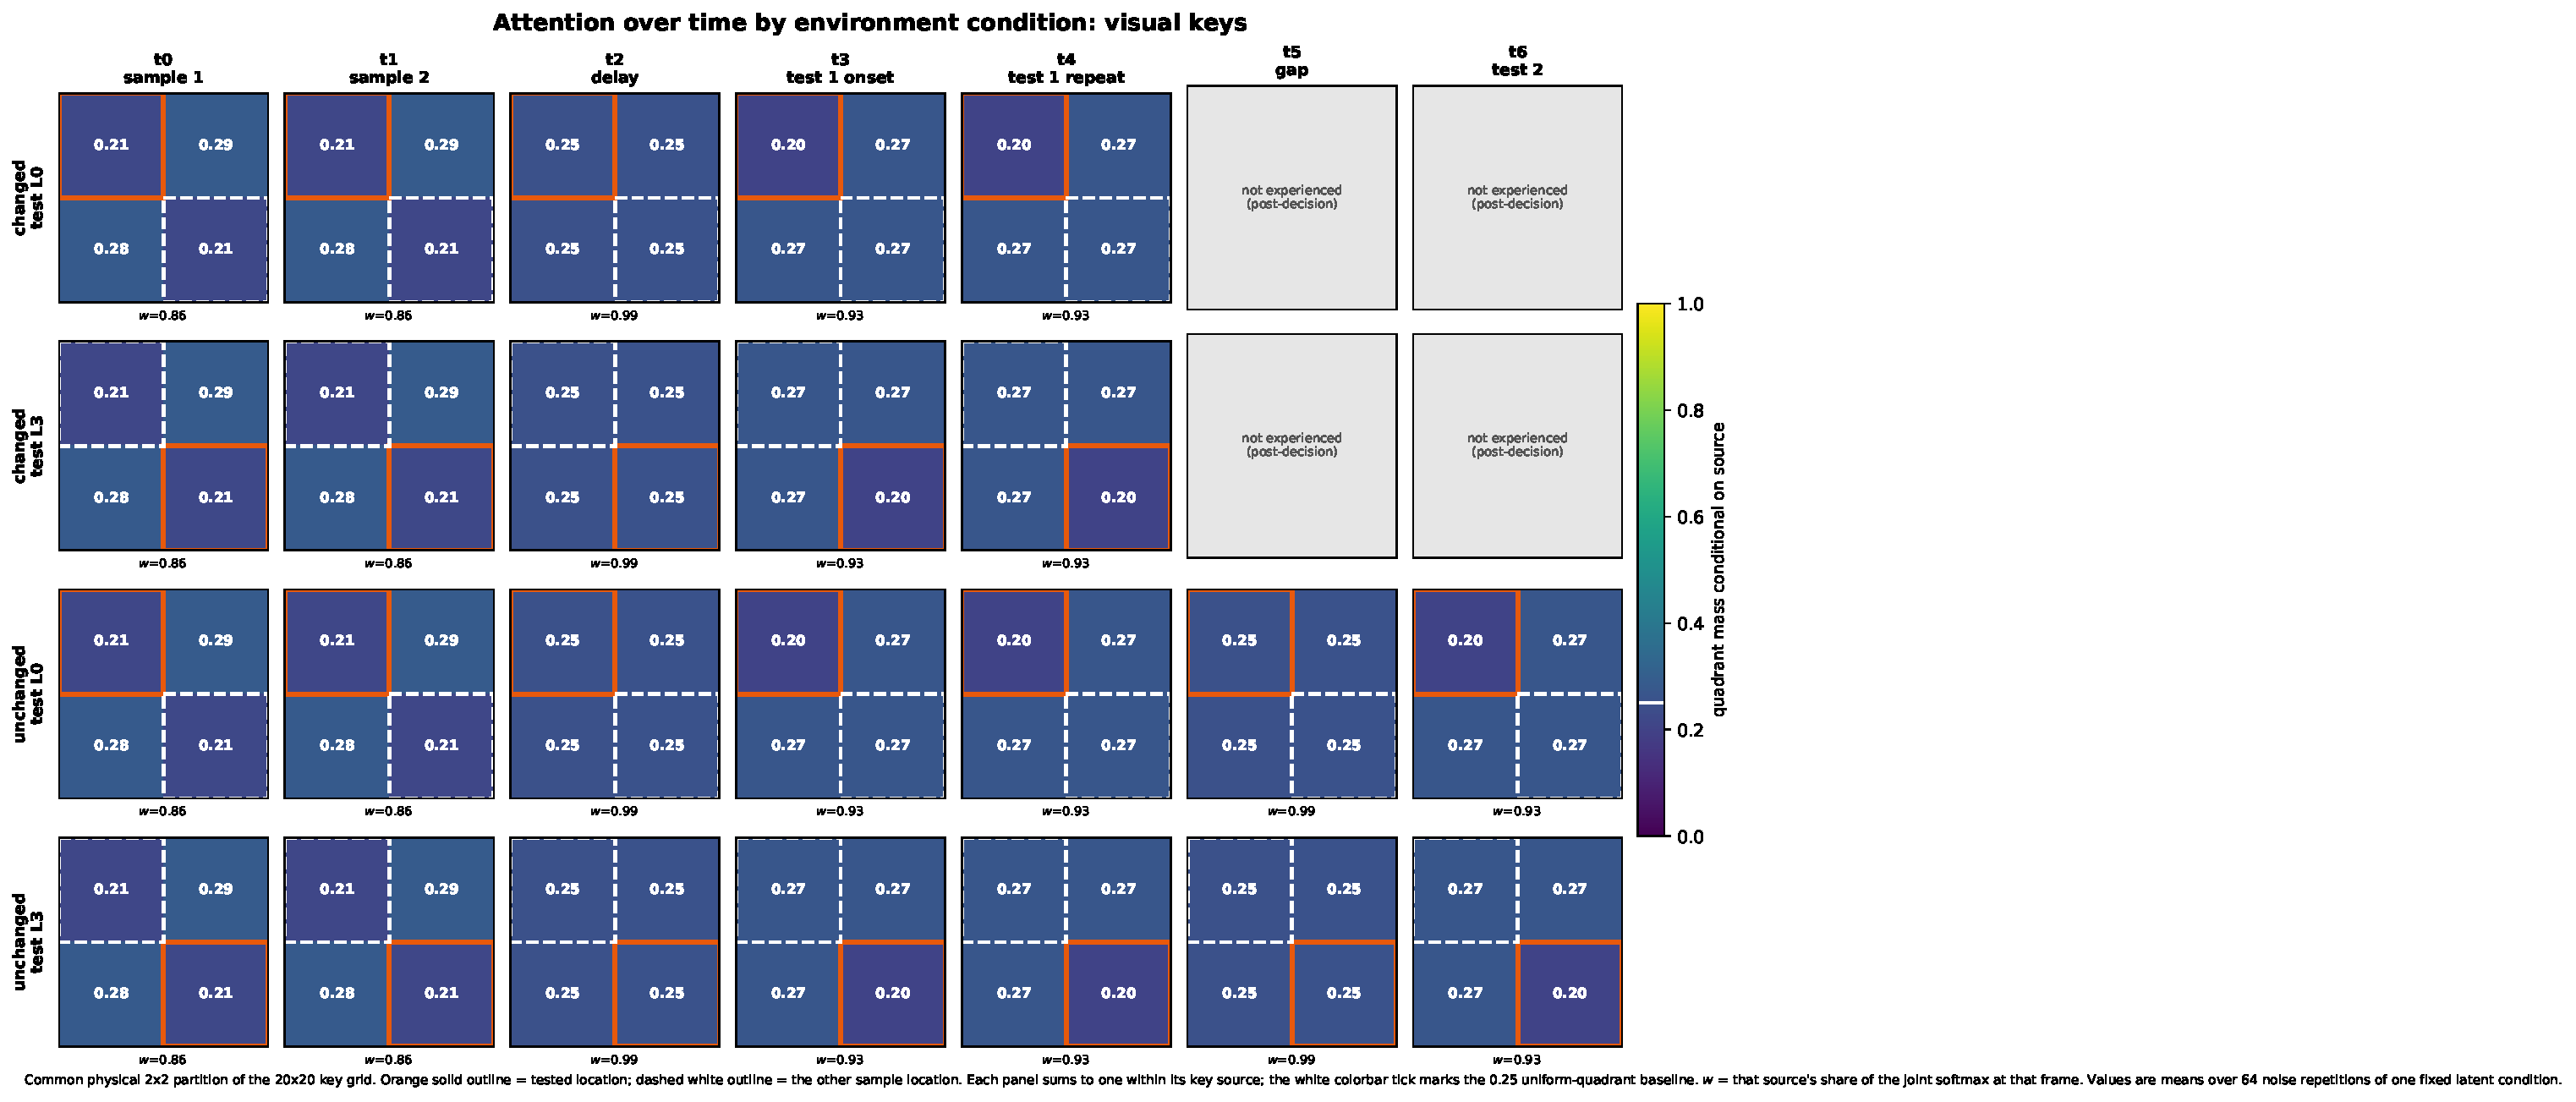
\includegraphics[width=0.97\textheight]{attention_time_condition_visual.pdf}
\caption{\textbf{Visual keys carry no condition-contingent spatial signal.} Rows are the four
environment conditions; columns are the seven frames. Each panel is the common physical
$2\times2$ partition of the $20\times20$ visual-key grid, coloured by quadrant mass
conditional on the visual source (each panel sums to one; the white tick on the colourbar is
the $0.25$ uniform baseline). Orange solid outline marks the tested location, dashed white
the other sample location, and $w$ below each panel is the visual share of the joint softmax.
Grey panels are frames that changed trials never experience, because the episode terminates
in the first-test window. The map is identical across rows and is set entirely by which
patches contain a Gabor --- which it avoids.}
\label{fig:visual}
\end{sidewaysfigure}

\begin{sidewaysfigure}
\centering
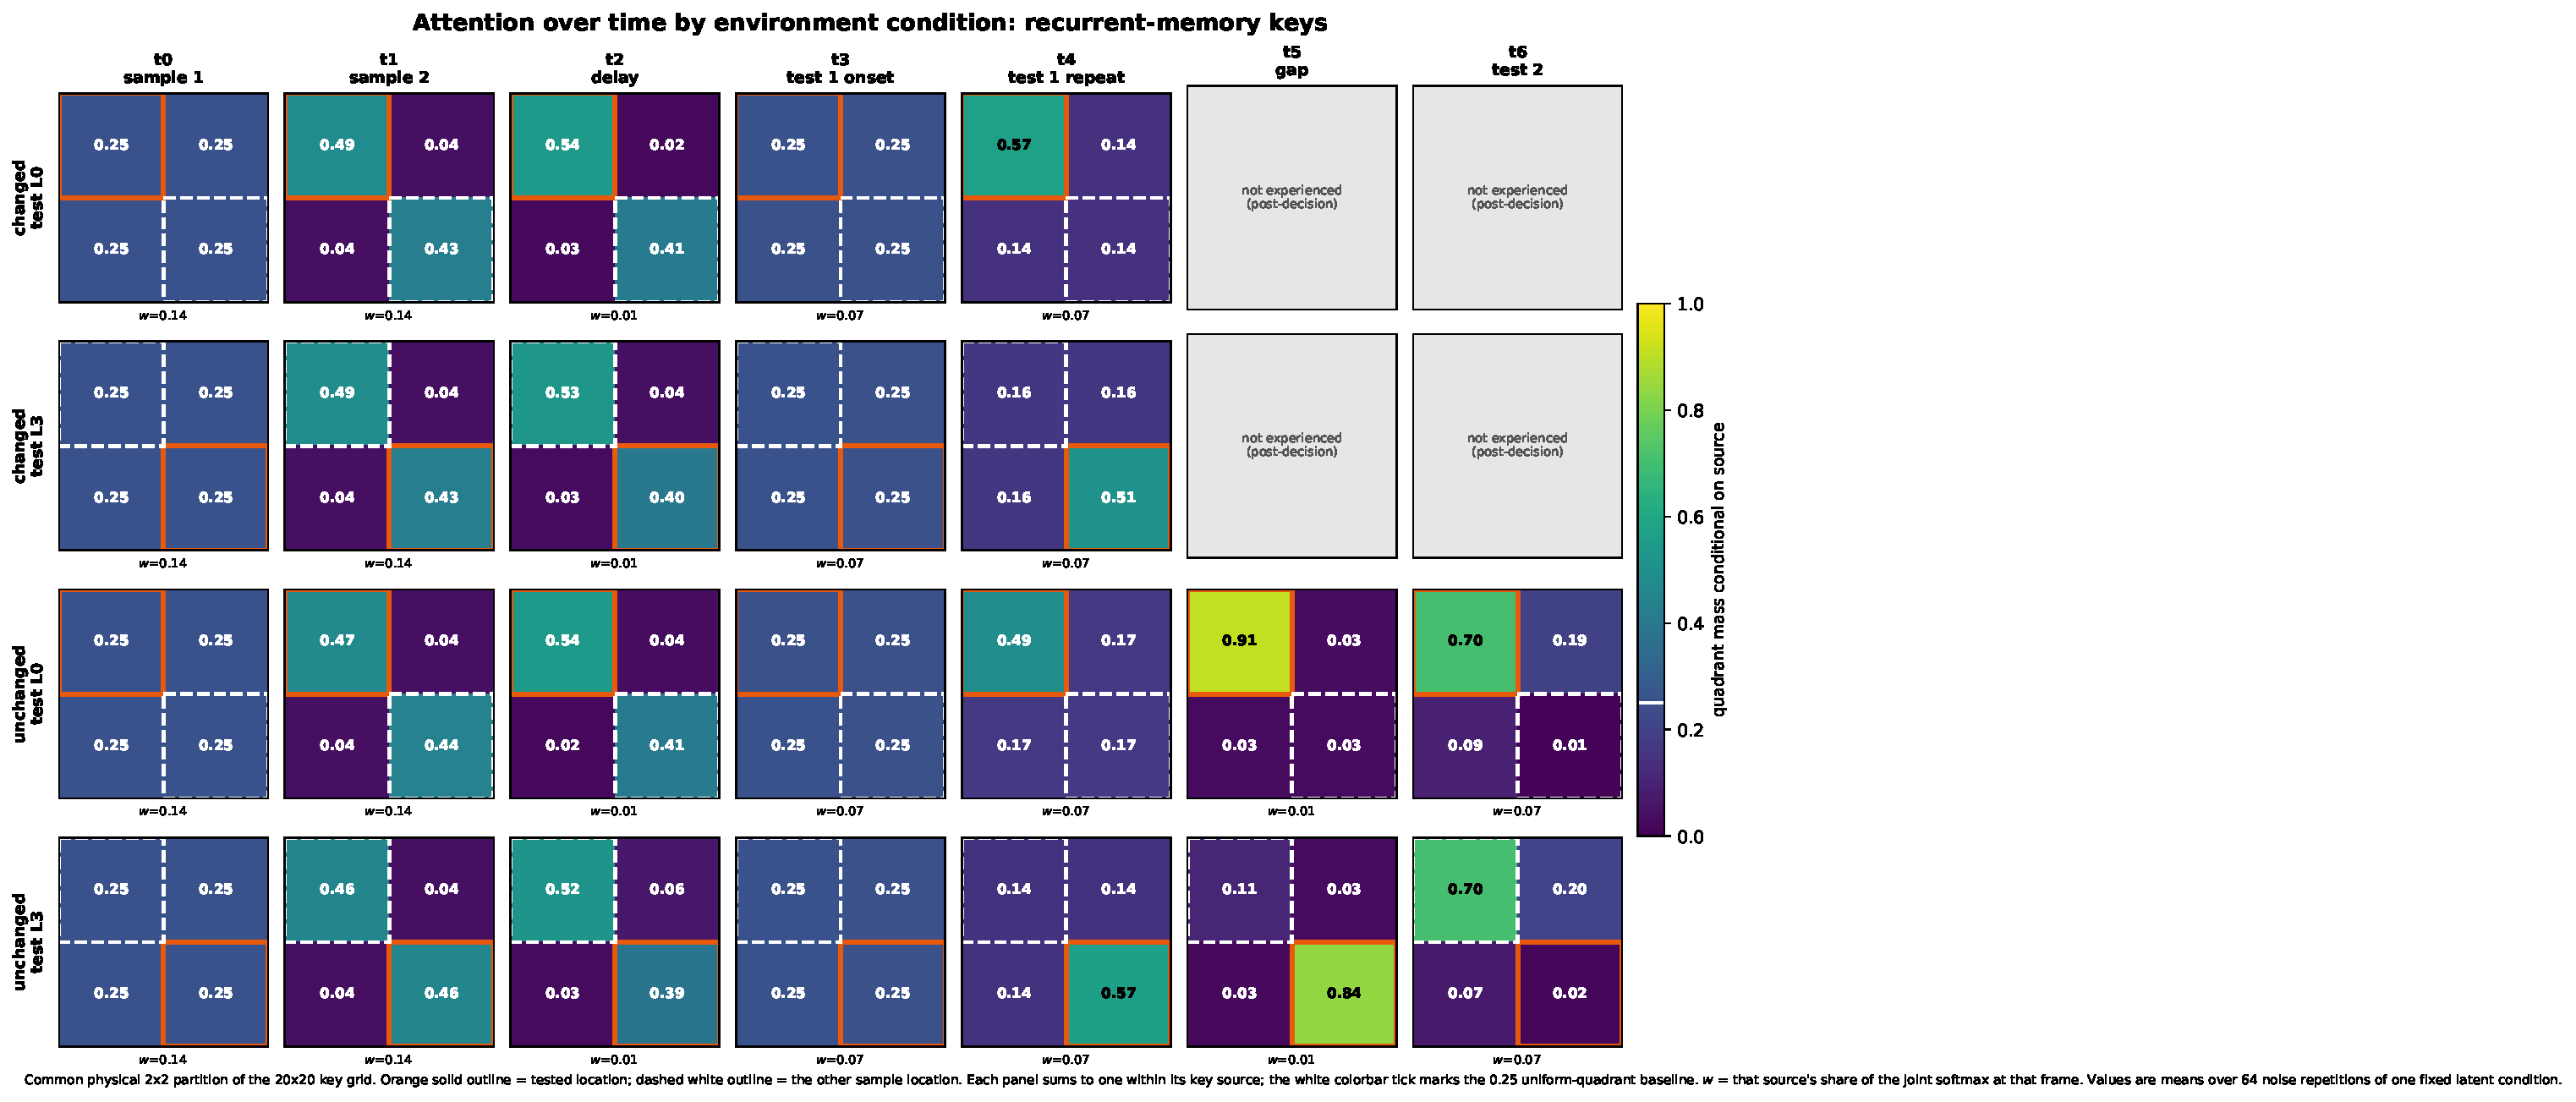
\includegraphics[width=0.97\textheight]{attention_time_condition_memory.pdf}
\caption{\textbf{Recurrent-memory keys encode, maintain, reset, and select.} Same layout,
scores, and outlines as Figure~\ref{fig:visual}, for the memory key block. Uniform at $t_0$
(the memory is zero-initialized), split across both sample quadrants at $t_1$--$t_2$,
near-uniform again at first-test onset $t_3$, tested-contingent at $t_4$ and through the gap
$t_5$, and --- critically --- locked to the top-left quadrant at $t_6$ irrespective of which
location was actually tested, which is what produces the sign reversal in the
tested-minus-other contrast.}
\label{fig:memory}
\end{sidewaysfigure}

\subsection{Memory keys: encode, maintain, reset, select}

Everything that varies over time or across conditions is in the memory block
(Figure~\ref{fig:memory}). Four stages are visible.

\paragraph{Encode.} At $t_0$ the memory map is exactly uniform ($0.250$ in all four
quadrants, in all four conditions), as it must be while the recurrent state is still
zero-initialized. By $t_1$ mass has moved onto \emph{both} sample quadrants ($0.43$--$0.49$
each) leaving $0.04$ in each blank quadrant. Both items are encoded, which is the correct
behaviour for a task with no cue.

\paragraph{Maintain.} At the blank delay $t_2$ the split persists ($0.52$--$0.54$ at L0,
$0.39$--$0.41$ at L3, $0.02$--$0.06$ in the blanks). This map is \emph{the same in all four
conditions}, including the two whose tested location is L3. The asymmetry is a fixed
location bias, not a prediction of the upcoming test --- which is the correct control, since
nothing in the display could support such a prediction.

\paragraph{Reset.} At first-test onset $t_3$ the quadrant map returns to $0.250$ in every
quadrant and every condition, and the tested-query same-minus-other contrast is zero to
floating-point precision in both sources. At token level the memory map at $t_3$ is not
literally uniform (coefficient of variation $0.10$ across the $400$ tokens, against $7.6$ at
$t_1$), but it is near-uniform enough that all quadrant structure disappears. The
maintained spatial code is discarded exactly when the test arrives, and rebuilt one frame
later.

\paragraph{Select.} At $t_4$ the memory concentrates on the tested location: $0.574$ and
$0.491$ at L0, $0.510$ and $0.566$ at L3, against $0.14$--$0.17$ at the other sample
location. The tested-location query shows the same thing, sending $+0.094$ to $+0.130$ more
memory mass to its own quadrant than to the other. On unchanged trials the concentration
strengthens through the blank gap $t_5$ ($0.907$ at L0, $0.839$ at L3) --- the only frame at
which routing is both strongly selective and almost entirely detached from the visual input,
since $w_M$ is only $0.010$ there.

\subsection{The selection is not location-general}

The apparent ``reselect the tested site'' story fails its control at the second test. At
$t_6$ both unchanged conditions route $0.70$ of their memory mass to the \emph{same}
quadrant, L0 --- which is the tested location in one condition and the untested location in
the other. The tested-minus-other contrast is therefore $+0.194$ when L0 is tested and
$-0.188$ when L3 is tested (Figure~\ref{fig:timecourse}, bottom row, third and fourth
columns; Table~\ref{tab:contrasts}). Averaged over locations this cancels to nearly zero,
which is exactly what the pooled estimate for this checkpoint reported
($+0.0015$, 95\% CI $[-0.050, +0.051]$, $n=64$).

This matters for how the $t_4$ and $t_5$ results should be read. At those frames the
selection genuinely follows the tested location and survives the L0/L3 control. At $t_6$ it
does not, and a location-collapsed analysis would have hidden that by averaging a positive
and a negative effect. \textbf{Reporting the tested-minus-other contrast separately at each
tested location is not a robustness check here; it is the difference between a real result
and an artefact.}

\begin{figure}[t]
\centering
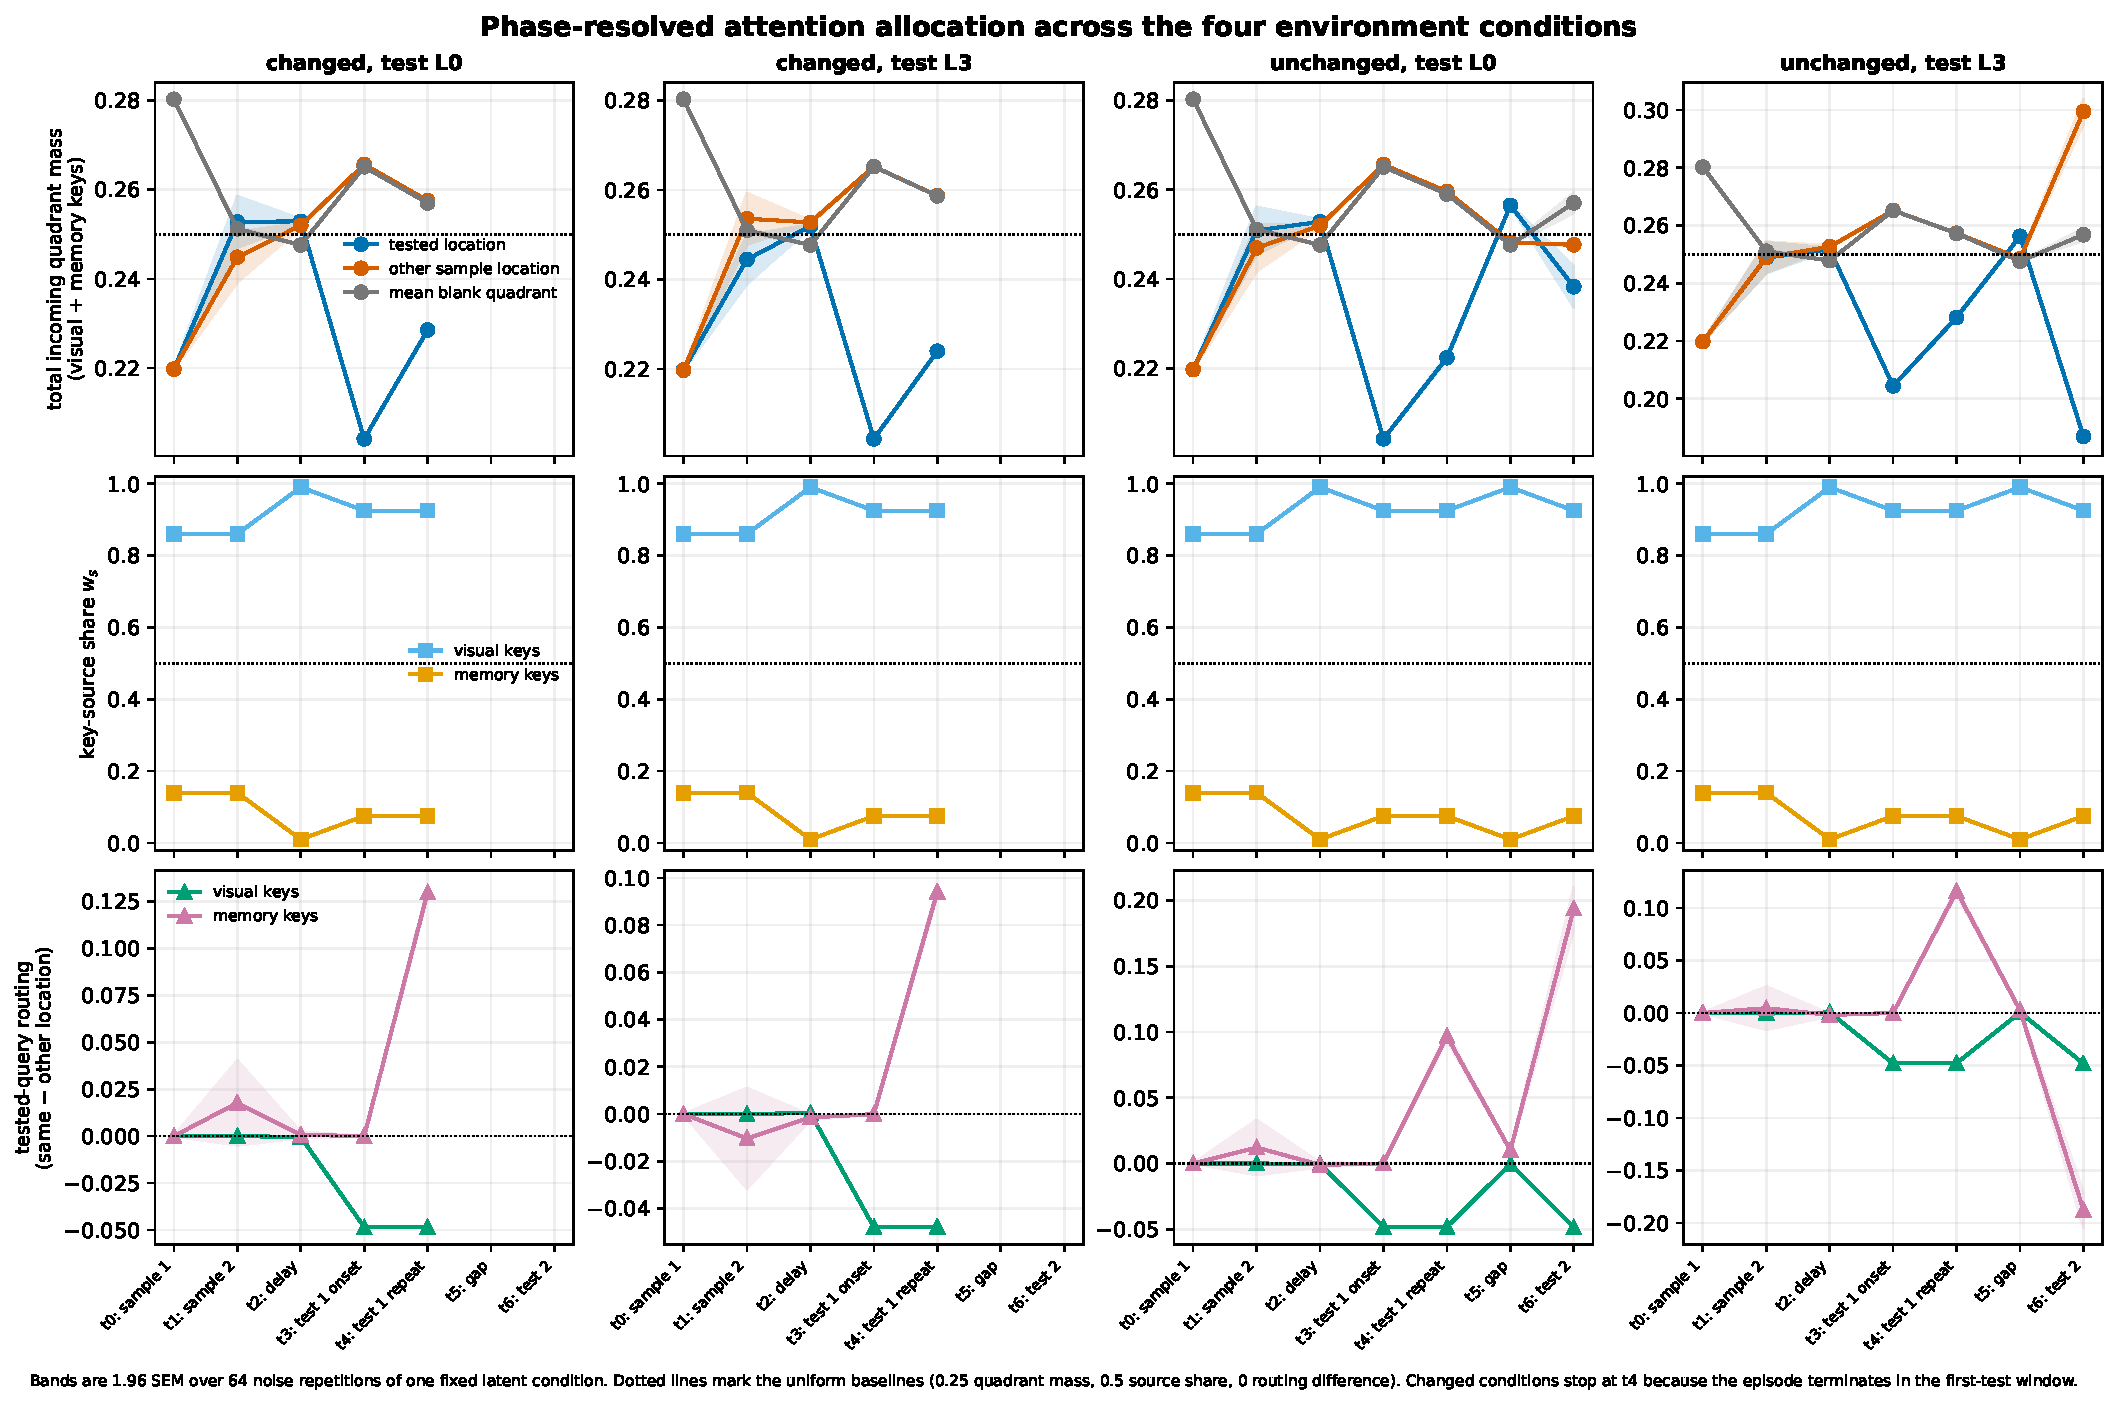
\includegraphics[width=\textwidth]{attention_timecourse_conditions.pdf}
\caption{\textbf{Phase-resolved allocation across the four environment conditions.} Top:
total incoming quadrant mass (visual $+$ memory) at the tested location, the other sample
location, and the mean blank quadrant; the dotted line is the $0.25$ uniform baseline. The
combined trace is dominated by the visual block and stays within $\pm0.05$ of uniform.
Middle: key-source share, which tracks the number of visible Gabors. Bottom: tested-location
query routing, same minus other location, per source; the memory trace rises at $t_4$ in all
conditions but reverses sign between the two tested locations at $t_6$. Bands are
$1.96$ SEM over $64$ noise repetitions of one fixed latent condition.}
\label{fig:timecourse}
\end{figure}

\begin{table}[t]
\centering
\small
\caption{Tested-minus-other location contrasts by frame and condition, from the
tested-location query. Visual routing is a constant $-0.048$ wherever a test stimulus is
present; memory routing is tested-contingent at $t_4$ (and at $t_5$, omitted here because
only the unchanged conditions reach it) but location-locked at $t_6$. Dashes are frames the
condition never experiences.}
\label{tab:contrasts}
\begin{tabularx}{\textwidth}{Y r r r r r r}
\toprule
Condition & Source & $t_1$ & $t_2$ & $t_3$ & $t_4$ & $t_6$\\
\midrule
changed, test L0   & visual & $0.000$ & $-0.000$ & $-0.049$ & $-0.048$ & ---\\
                   & memory & $+0.018$ & $+0.001$ & $0.000$ & $+0.130$ & ---\\
changed, test L3   & visual & $0.000$ & $+0.000$ & $-0.048$ & $-0.048$ & ---\\
                   & memory & $-0.010$ & $-0.001$ & $-0.000$ & $+0.094$ & ---\\
unchanged, test L0 & visual & $-0.000$ & $-0.000$ & $-0.048$ & $-0.048$ & $-0.049$\\
                   & memory & $+0.012$ & $-0.001$ & $-0.000$ & $+0.097$ & $\mathbf{+0.194}$\\
unchanged, test L3 & visual & $0.000$ & $+0.000$ & $-0.048$ & $-0.048$ & $-0.048$\\
                   & memory & $+0.005$ & $-0.002$ & $-0.000$ & $+0.116$ & $\mathbf{-0.188}$\\
\bottomrule
\end{tabularx}
\end{table}

\subsection{None of this is shown to be response-causal}

A companion intervention on the same frozen checkpoint applied a $-6$ additive key-logit
bias at the future-tested quadrant during the two sample frames. The manipulation worked as
a routing manipulation: mean attention mass at that quadrant fell from $0.2342$ to $0.0011$.
It did nothing behaviourally. Across $704$ matched trial pairs there were \emph{zero}
discordant correctness outcomes, giving an observed $\Delta$ accuracy of $+0.000$; because
the paired bootstrap is degenerate when every pair agrees, the conservative two-sided
no-discordance bound is $|\Delta\text{accuracy}| < 0.0052$. The identical operation at the
other active sample and at a blank control quadrant was equally inert. Hit rate, $d'$, and
mean hit frame were unchanged at every probe magnitude.

Sample-phase spatial allocation in this checkpoint is therefore descriptive routing evidence
and nothing more. The measured maps are real and highly reproducible under noise, but the
one causal test we ran says the agent's first-test decision does not depend on them.

\section{Discussion}

Three things are worth carrying forward.

\textbf{Source separation is doing the work.} If the visual and memory key blocks are summed
before reduction --- the co-located ``V$+$M'' diagnostic --- the entire memory story is
buried under a visual block that is $6$ to $99$ times larger and carries no
condition-contingent signal. The combined trace in the top row of
Figure~\ref{fig:timecourse} never leaves a $\pm0.05$ band around uniform, while the memory
block underneath it swings from $0.25$ to $0.91$. The VDA-series convention of splitting
sources before query reduction is what makes the effect visible, and this is a sharper
demonstration of that than any cued case we have run.

\textbf{The reset at $t_3$ is the most interesting unexplained observation.} A recurrent
memory that has held a two-item spatial code across a blank delay discards its quadrant
structure at the exact frame the test appears, then rebuilds a one-item, tested-location code
one frame later. We do not know whether this is a genuine computational stage --- clear the
maintained code, then write the comparison --- or an incidental consequence of the memory
update being dominated by the new visual input. Distinguishing those requires reading the
recurrent state directly rather than the attention over it.

\textbf{Uncued does not mean unselective, but it does raise the evidential bar.} Without a
cue there is no experimenter-named location to align routing to before the test, so the only
defensible spatial contrasts are post-test ones, and they must be reported per tested
location. The $t_6$ reversal shows what happens otherwise.

The obvious next experiments are (i) a corrected-contract retrain, without which none of the
above can be promoted past provenance; (ii) clamping at $t_4$--$t_5$ rather than at the sample
frames, since that is where the tested-contingent signal actually is; and (iii) a linear
probe on the recurrent state at $t_2$ and $t_3$ to test whether the maintained code really is
discarded or merely becomes invisible to attention.

\section{Validity and provenance}\label{sec:validity}

\textcolor{WarnRed}{\textbf{This checkpoint lineage is marked invalid for behavioural claims
under the corrected Luo task contract.}} The enforced contract requires each sample
orientation to be drawn independently from $\mathrm{Uniform}[0^\circ,180^\circ)$ on every
trial, with the signed change drawn from $\mathrm{Uniform}(-\theta,\theta)$ and $\theta$
controlling only the maximum absolute change. The frozen checkpoint records fixed session
base orientations ($98.79^\circ$ at L0, $128.73^\circ$ at L3) and carries no
\texttt{orientation\_sampling} marker, so it was trained under the earlier
fixed-pair, curriculum-coupled generator. Its producer script now refuses that checkpoint
outright. The consequences for this report are specific:

\begin{itemize}
\item Sample orientations were near-constant across training, so the recurrent memory had far
less to encode than the corrected task demands. The encode/maintain stages in
Figure~\ref{fig:memory} may reflect a memorized pair rather than trial-specific storage.
\item No d$'$, criterion, psychometric, lesion, or Luo-replication claim from this lineage is
admissible, including the behavioural curves in Figure~\ref{fig:behaviour}, which are
reproduced here only to locate the $18^\circ$ attention probe.
\item Warm-starting a corrected run from this checkpoint would contaminate it. A neutral
parent must be retrained from scratch.
\end{itemize}

\vspace{6pt}
\noindent What does survive is the measurement methodology and the qualitative dissociation it
exposes: source-split, per-frame, per-condition, survivor-controlled quadrant maps, displayed
on a common physical partition with an explicit uniform baseline and an explicit source
share. Those conventions transfer unchanged to the corrected retrain, and the analysis in
this report can be regenerated against it by pointing the same producer at the new assay
directory.

Additional boundaries that hold regardless of the contract issue: the intervals are over
noise repetitions of one fixed latent condition at one checkpoint, not over training seeds or
over the trial distribution; attention weights are normalized routing, not orientation-content
decoding; the $-6$ logit bias is strong soft suppression rather than hard exclusion, leaving
$0.48\%$ of natural target-region mass; and the biological comparison target,
Luo and Maunsell (2015) V4, is a reference point for the task design only --- no
neural-equivalence claim is made anywhere in this report.

\section*{Reproduction}

All figures are produced by
\texttt{analysis/make\_luo2015\_vda\_style\_attention\_figs.py}, which reads the frozen
\texttt{fixed\_condition\_attention.npz} cache from
\texttt{reports/luo2015\_scientific\_assay\_20260803\_production} and writes
\texttt{figure\_statistics.json} alongside them. It re-runs no checkpoint and trains nothing.
Every number quoted in this report appears in that JSON file or in the assay's
\texttt{data/summary.json}.

\end{document}
